\documentclass[aspectratio=43,10pt,fleqn,t]{beamer}
\usepackage[fhgindent,theme=default]{beamerfhg}
\usepackage{eurosym}
\usepackage{polyglossia}
\setdefaultlanguage{english}
\usepackage[autostyle,german=guillemets]{csquotes}
\usepackage[linesnumbered,ruled,vlined]{algorithm2e}

\usepackage{xcolor}
\usepackage{listings}
\usepackage{caption}
\DeclareCaptionFont{white}{\color{white}}
\DeclareCaptionFormat{listing}{%
	\parbox{\textwidth}{\colorbox{gray}{\parbox{\textwidth}{#1#2#3}}\vskip-4pt}}
\captionsetup[lstlisting]{format=listing,labelfont=white,textfont=white}
\lstset{frame=lrb,xleftmargin=\fboxsep,xrightmargin=-\fboxsep}

\lstset{
	% numbers=left,
	breaklines=true,
	% backgroundcolor=\color{light-gray},
	tabsize=4,
	% basicstyle=\ttfamily,
	literate={\ \ }{{\ }}1	
}




\title{Compliant Manipulation using Reinforcement Learning guided by Task Specification}
\subtitle{Master Thesis}
\author{Abhishek Padalkar}
\begin{document}

\titlebackgroundtrue
\begin{frame}[plain]
 \titlepage
 \centering
 
\includegraphics[scale=0.5]{FKIE-logo}
\end{frame}
\titlebackgroundfalse


\section{Introduction}
\subsection{Motivation}

\begin{frame}{Motivation}
\begin{itemize}
	\item Most of the real world robotic manipulation tasks present the need for compliant manipulation.

	\item Robot needs to respond to the contact forces while executing the task.
	
	\item Classical planning and control algorithm fail to perform satisfactorily due to the lack of precise model of contact forces and high computational complexity. 
	
	\item Reinforcement learning can learn the compliant manipulation task but requires high number of interactions.
	
	\item Accuracy of simulations affects the learned behavior.
\end{itemize}
\end{frame}

\subsection{Problem Statement}

\begin{frame}{Problem Statement}
Develop a learning based approach for achieving compliant manipulation that allows to exploit partial/incomplete models of the task and the environment provided by the task specification.
\vspace{0.5cm}

We plan to solve above problem by dividing the problem into two sub-problems:
\begin{itemize}
	\item Model the available knowledge about task and environment using existing task specification framework.

	\item Use RL for learning gradually more complete and robust action models for compliant and repetitive manipulation tasks.
\end{itemize}


	We demonstrate our approach by learning demo tasks of
\begin{itemize}
	\item Opening door, and
	\item Cutting vegetables.
\end{itemize}
\end{frame}

\begin{frame}
	\begin{figure}
		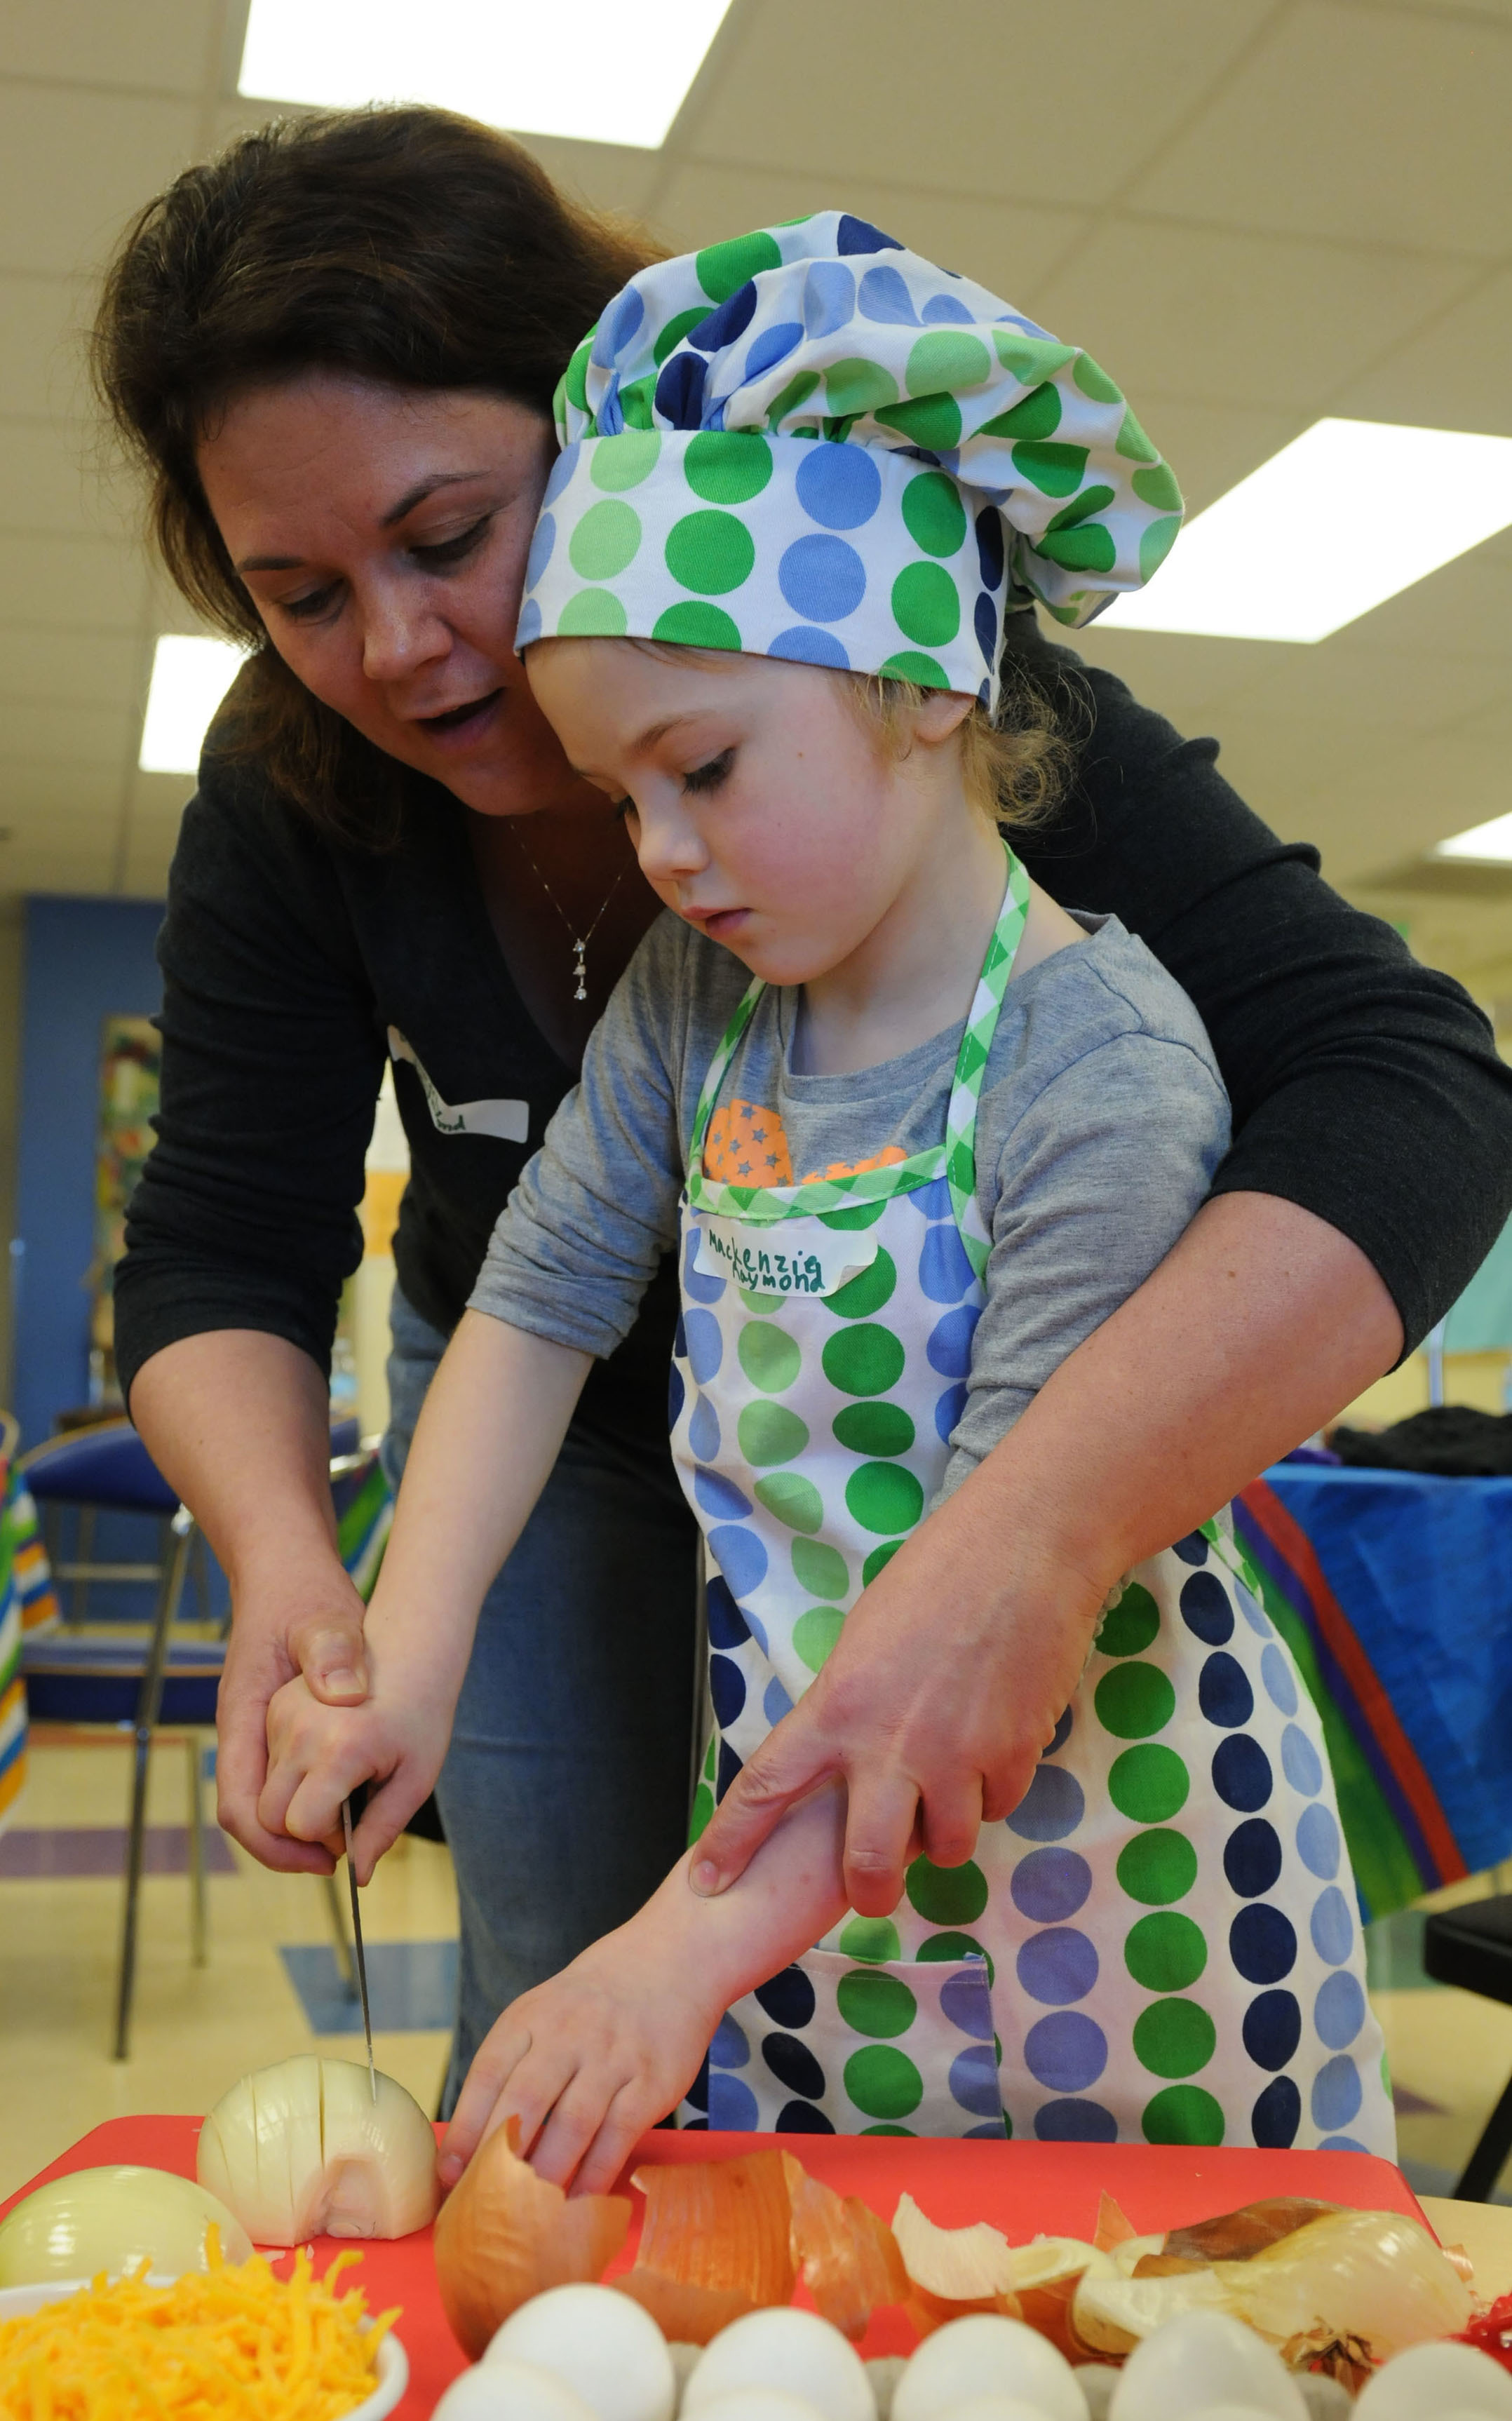
\includegraphics[width=0.41\textwidth]{images/mother_child}
		\caption{Mother teaching child to cut vegetables}
	\end{figure}
	\end{frame}
\section{Related Work}

\begin{frame}[fragile]{Related Work}{\small Task Specification in KUKA Robot Language}
	
	\begin{lstlisting}[label=KRL-sample,caption=KRL code]
    INI
    PTP HOME ; go to HOME joint configuration
    LIN P1   ; linear motion to point P1
    LIN P2   ; linear motion to point P2
\end{lstlisting}
	\begin{itemize}
		\item Heavily used in industrial settings 
		\item Reliable
		\item Difficult to integrate sensory feedbacks
		\item Limited expressive power \cite{leidner2017cognitive}
	\end{itemize}
\end{frame}


\begin{frame}[fragile]{~}{Task Specification using Task Frame Formalism \cite{mason1981compliance}}
	
	\begin{lstlisting}[label=tff,caption=Task Specification using TFF: Open Door]
    move compliantly {
        with task frame directions
        xt: force 0 N
        yt: force 0 N
        zt: velocity v mm/sec
        axt: force 0 Nmm
        ayt: force 0 Nmm
        azt: force 0 Nmm
    } until distance > d mm
    \end{lstlisting}
	
	\begin{itemize}
		\item Using hybrid control, various control modes are assigned to each axis of the \textit{task frame} or \textit{compliance frame} \cite{nagele2018prototype}. 
	\end{itemize}
\end{frame}

\begin{frame}[fragile]{~}{Other Task Specification \cite{leidner2017cognitive}}
	\begin{itemize}
		\item Leidner presents symbolic representation of the task in PDDL along with the geometric representation of the task using sequence of low level movement sequences needed to complete the action. 
		\item iTaSC synthesizes control inputs based on provided task space constraints \cite{DeSchutter-ijrr2007, DecreBruyninckxDeSchutter2013, decre09}. 
		\item It formulates an optimization problem considering provided constraints in the environment. 
 
	\end{itemize}
\end{frame}

\begin{frame}{~}{Reinforcement Learning}
	\begin{itemize}
		\item \textcolor{fhggreen}{Model-based} reinforcement learning learns the model of environment as well as policy for performing the task.
		\item Number of interactions required can be very high for learning model of the environment.
		\item \textcolor{fhggreen}{Model-free} reinforcement learns policy required for achieving the task without learning the model of the environment. 
		\item Model-free reinforcement learning algorithms require less number of interactions.
	\end{itemize}
\end{frame}

\begin{frame}{~}{Policy Search Methods}
	\begin{itemize}
		\item Policy search methods are model-free learning methods which directly learn policy to take action in current observable state without learning value function.
		\item Policy search methods are used heavily in robot control due to their ability to handle high dimensional state-action space.
		\item Algorithms:
		\begin{itemize}
			\small
			\item Finite difference method : Learns by comparing returns with baseline after exploration in parameter space.
			\item Likelihood ratio method / REINFORCE : Uses policy gradient theorem  
			\item Natural actor critic algorithm 
			\item Path integral policy improvement (PI$^{2}$)
			\item Expectation-maximization method (PoWER) : Learns by exploration in the parameter space and by weighing the exploration by returns
		\end{itemize} 

	\end{itemize}
\end{frame}

\begin{frame}{~}
	\textbf{Door opening task}
			\begin{itemize}
	\item Motion synthesis using the geometric model of the door : requires accurate model of door
	\item Adaptive control along with on-line estimation of the door parameters using force-torque sensors : sensor noise affects the parameter estimation
	\item Learning force policies using reinforcement learning : requires numerous interactions with environment
	\item Learning the task from human demonstrations using Dynamic Motion Primitives : not generalizable for different doors
\end{itemize}

\textbf{Vegetable cutting task}
\begin{itemize}
	\item Deep recurrent neural network with model predictive control : requires large amount of data to learn the model 
	\item Using sequence of Dynamic Motion Primitives : purely motion-based approach
\end{itemize}
\end{frame}

\section{Solution}
\begin{frame}{Solution}{\small Approach}
	\begin{itemize}
		\small
	\item Provide task specification using Task Frame Formalism (TFF), which also contains a policy to be learned by reinforcement leaning for generating control commands.

	\item Design policy for control command generation in the task specification. This policy can be a engineered policy for a well understood problem or can be a generic parameterized policy e.g. neural network or radial basis function network.

	\item Design a reward function for the given task.

	\item Use existing reinforcement learning methods to learn parameters of the policy to maximize given reward function by carrying out trials in the environment.
	\end{itemize}
\end{frame}
\begin{frame}{Solution}{\small Components}
	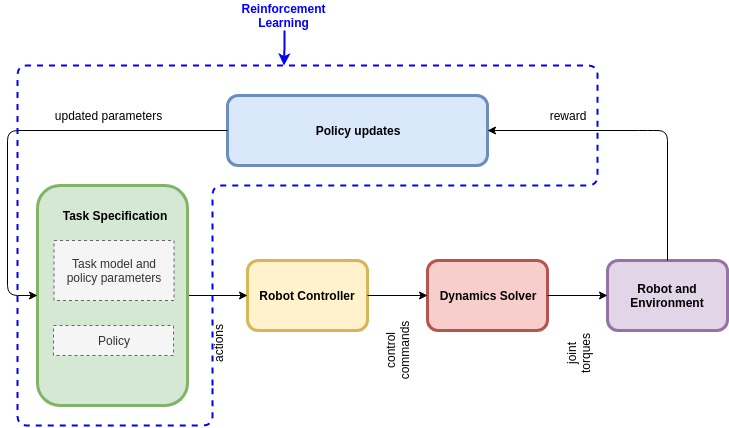
\includegraphics[width=\textwidth]{images/composition}
\end{frame}

\begin{frame}{Task Frame Formalism}
	Task frame formalism provides guidelines for identifying reciprocal degrees of freedom and task specification using them.
	
	\newgeometry{textwidth=11.53cm}%
	%\vskip1ex
	\begin{minipage}[b]{0.49\textwidth}
		
		\begin{figure}
				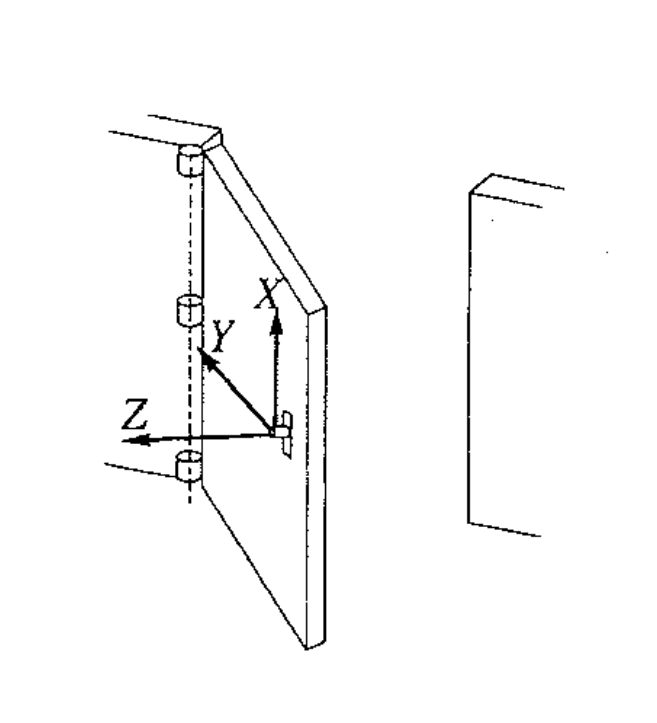
\includegraphics[width=0.8\textwidth]{images/tff_open_doora.png}
			\caption{\scriptsize Task frame selection for door opening task}
		\end{figure}
	\end{minipage}
	\hfill
	\begin{minipage}[b]{0.49\textwidth}
				\begin{figure}
				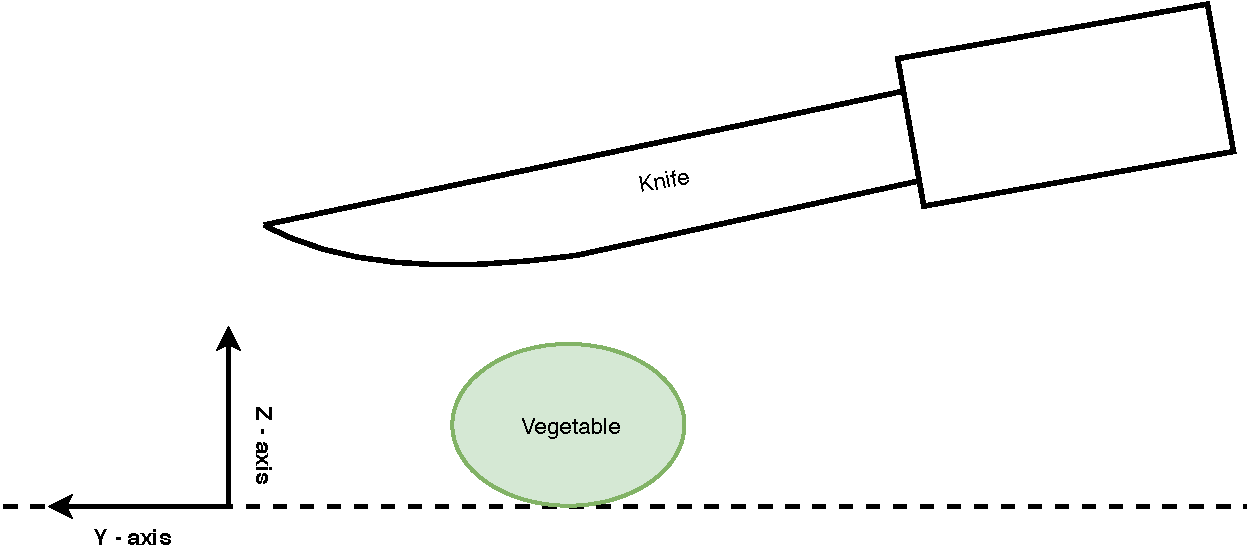
\includegraphics[width=0.8\textwidth]{images/tff_knife}
				\vspace{1.5cm}
				\caption{\scriptsize Task frame selection for vegetable cutting task}
				\end{figure}
	\end{minipage}
\end{frame}

\begin{frame}[fragile]{~}{Task Specification for opening door}
\begin{figure}
\begin{lstlisting}[label=tff-open-door-a,caption=Task Specification using TFF: Open Door]
    move compliantly {
        with task frame directions
        xt: force 0 N
        yt: force 0 N
        zt: velocity v m/sec
        axt: force 0 Nm
        ayt: force 0 Nm
        azt: force 0 Nm
    } until chord length > d m or force z > f N
\end{lstlisting}
	\end{figure}
\end{frame}

\begin{frame}[fragile]{~}{Task Specification for cutting vegetables}
		\begin{figure}
\begin{lstlisting}[label=cut_vegies,caption=Cut vegetables]
    move compliantly {
        with task frame directions
        xt: velocity 0 m/s 
        yt: velocity v(t) m/s
        zt: force f(environment, robot, task) N
        axt: velocity 0 rad/s
        ayt: velocity 0 rad/s
        azt: velocity 0 rad/s
    }until distance y > d m			
\end{lstlisting}
		\end{figure}
\end{frame}

\begin{frame}{Reinforcement Learning Algorithms}{\small REINFORCE}
		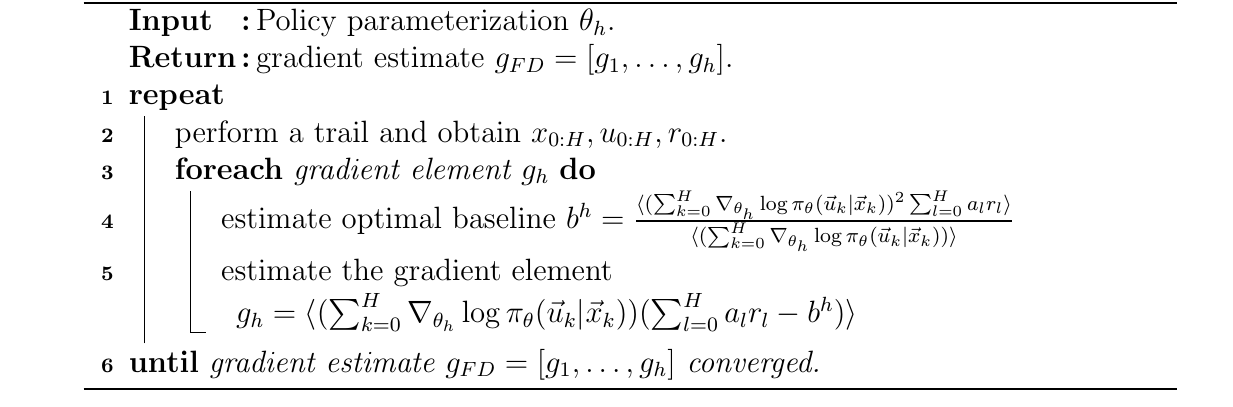
\includegraphics[width=\textwidth]{images/reinforce}
		
		\begin{itemize}
			\small
			\item Uses policy gradient theorem to estimate the gradient of the parameters.
			\item Adds exploration noise in the actions at every discrete time step.
		\end{itemize}
\end{frame}

\begin{frame}{~}{\small Policy learning by Weighting Exploration with the Returns (PoWER).}
	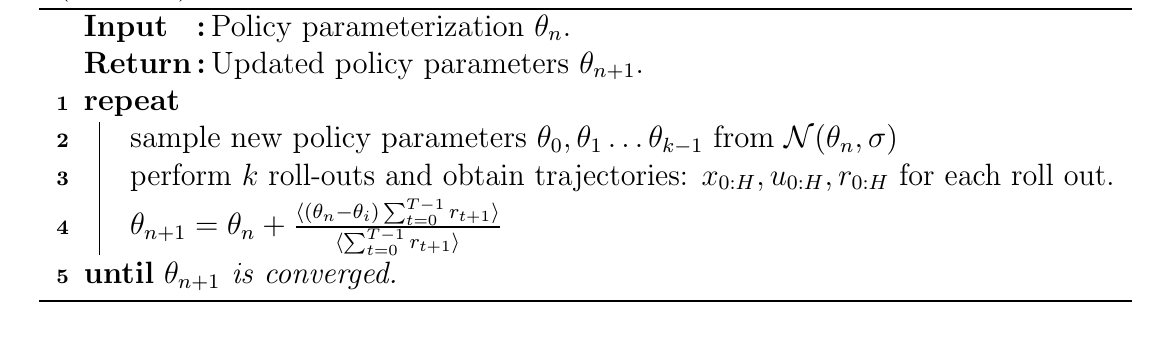
\includegraphics[width=\textwidth]{images/power}

\begin{itemize}
	\small 
	\item Uses expectation-maximization method to estimate the gradient of the parameters.
	\item Adds exploration in the parameters at the beginning of the episode.
\end{itemize}
\end{frame}

\begin{frame}{Policy Representation}
	\begin{itemize}
		\item Linear policy \begin{align}
		f = -(A\dot{y} + B(0.5^{2} - (0.5 - \phi_{y})^{2}) + C(1-\phi_{z}))
		\end{align}
		\item Gaussian policy 
			\begin{align}
			f &= -(A\dot{y} + B(0.5^{2} - (0.5 - \phi_{y}^{2})) + \sum_{i=0}^{N-1}W\psi_{i}(\phi_{z})) \text{, and}\\
			\psi_{i}(\phi_{z}) &= \frac{1}{\sqrt{2\pi\sigma^{2}}}e^{\frac{(c_{i} - \phi_{z})}{2\sigma^{2}}},
			\end{align}
	\end{itemize}
	\small
	where $A, B, C$ are policy parameters,\\
	$\phi_{y}$ and $\phi_{z}$ are cutting phases in Y 
	and Z direction respectively \\ 
	$W$ is weight vector, \\
	$N$ is number of Gaussian functions,\\
	$c_{i}$ is the center of $i^{th}$ Gaussian, and \\
	$\sigma$ is width of Gaussian functions.
\end{frame}

\begin{frame}{Experimental Results}{\small Door opening task}
	\vspace{-0.5cm}
Experiments were performed with two robots:
\begin{itemize}
	\small
	\item Schunk LWA4D equipped with Schunk FTM115 force torque module and Schunk Dexterous Hand 
	\item Toyota Human Service Robot (HSR)
\end{itemize}
	\centering
	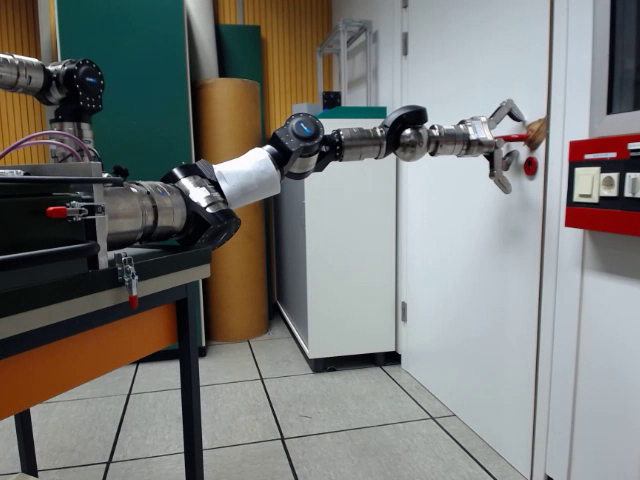
\includegraphics[width=0.52\textwidth]{images/exp/lwa_door}
	\hfil
	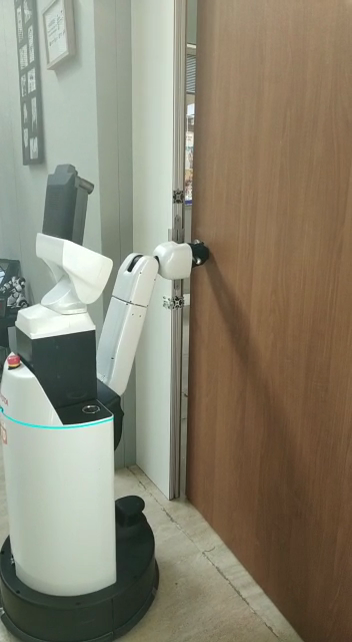
\includegraphics[width=0.25\textwidth]{images/exp/hsr_door} 
\end{frame}

\begin{frame}{~}{\small Schunk LWA4D opening unlatched door}
	\vspace{-1cm}
\begin{figure}[h]
	\centering
	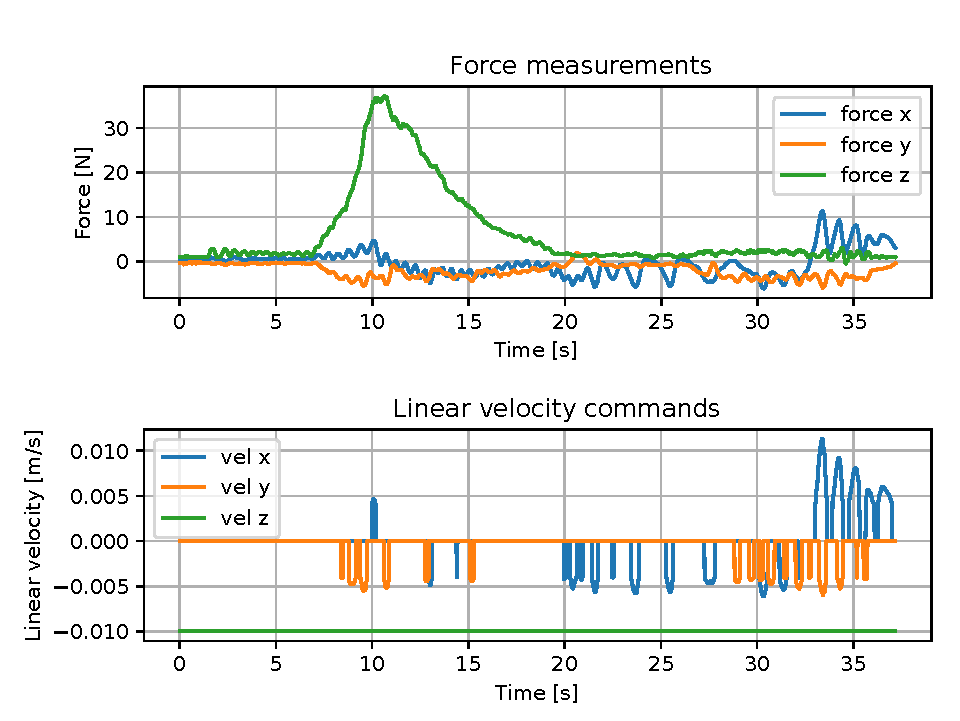
\includegraphics[width=0.8\textwidth]{images/exp/f-vn.pdf}
	\caption{Force readings at TCP and linear velocity applied to TCP}
	\label{EX:f-v}
\end{figure}
\end{frame}


\begin{frame}{~}{\small Schunk LWA4D opening unlatched door}
	\vspace{-1cm}
	\begin{figure}[t]
		\centering
		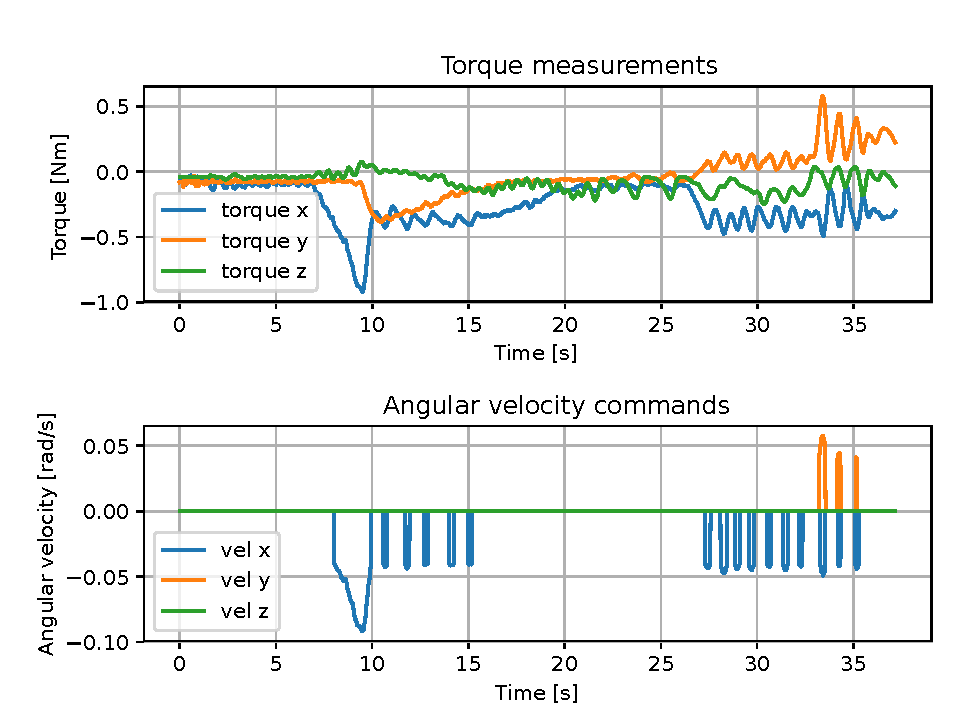
\includegraphics[width=0.8\textwidth]{images/exp/t-wn.pdf}
		\caption{Torque readings at TCP and velocity angular velocity applied at TCP}
		\label{EX:t-w}
	\end{figure}
\end{frame}

\begin{frame}{~}{\small Schunk LWA4D opening unlatched door}
	\vspace{-1cm}
	\begin{figure}[t]
		\centering
		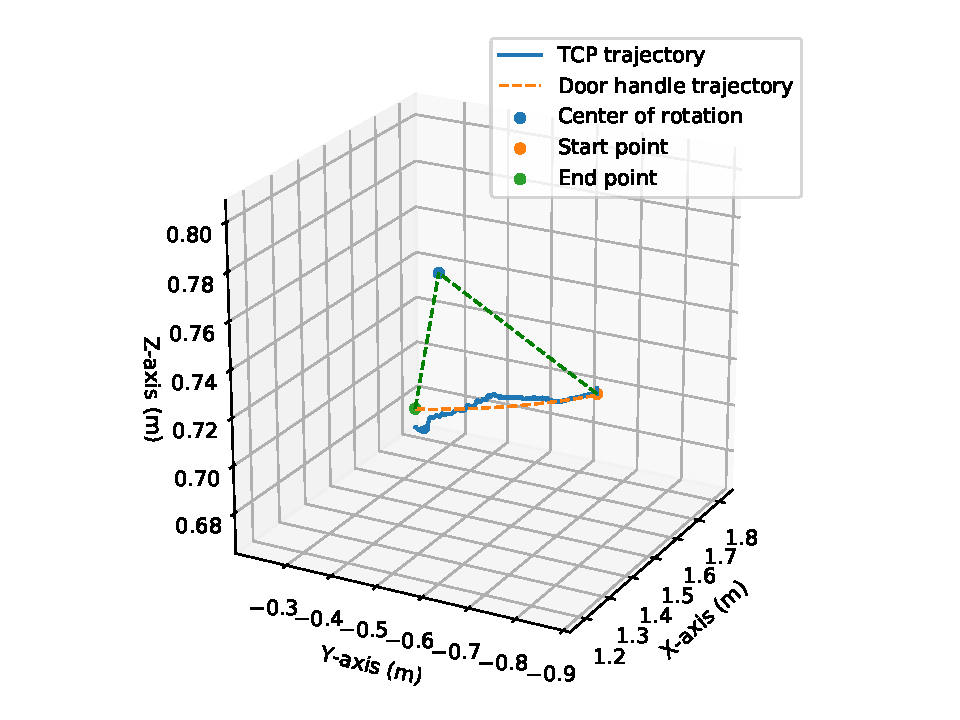
\includegraphics[width=0.8\textwidth]{images/exp/traj.pdf}
		\caption{Geometric analysis of trajectory traced by TCP}
		\label{EX:traj}
	\end{figure}
\end{frame}

\begin{frame}{~}{\small Toyota HSR trying to open jammed door}
	\vspace{-1cm}
	\begin{figure}[h]
		\centering
		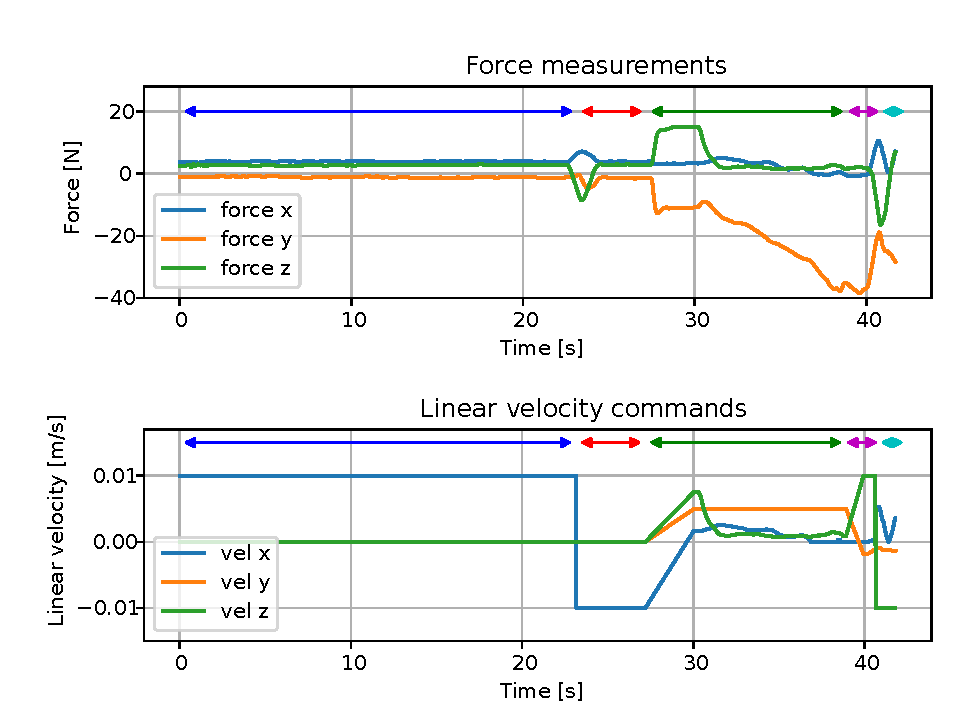
\includegraphics[width=0.8\textwidth]{images/exp/8776_fn.pdf}
		\caption{Force readings at TCP and linear velocity applied to TCP}
	\end{figure}
\end{frame}


\begin{frame}{~}{\small Toyota HSR trying to open jammed door}
	\vspace{-1cm}
	\begin{figure}[t]
		\centering
		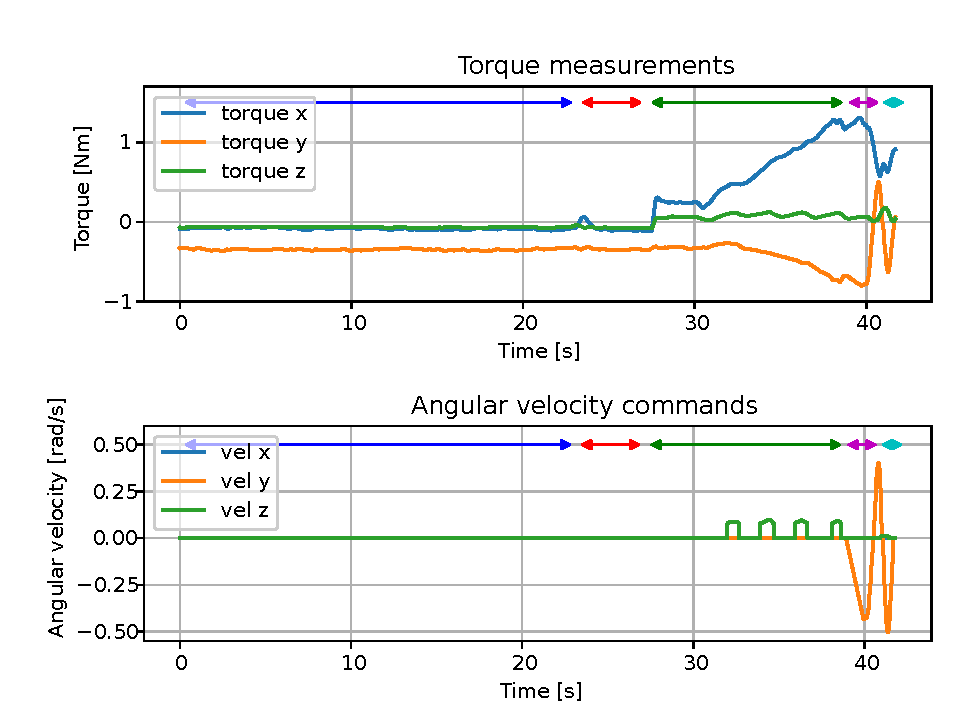
\includegraphics[width=0.8\textwidth]{images/exp/8776n.pdf}
		\caption{Torque readings at TCP and velocity angular velocity applied at TCP}

	\end{figure}
\end{frame}

\begin{frame}{~}{\small Toyota HSR trying to open jammed door}
	\vspace{-1cm}
	\begin{figure}[t]
		\centering
		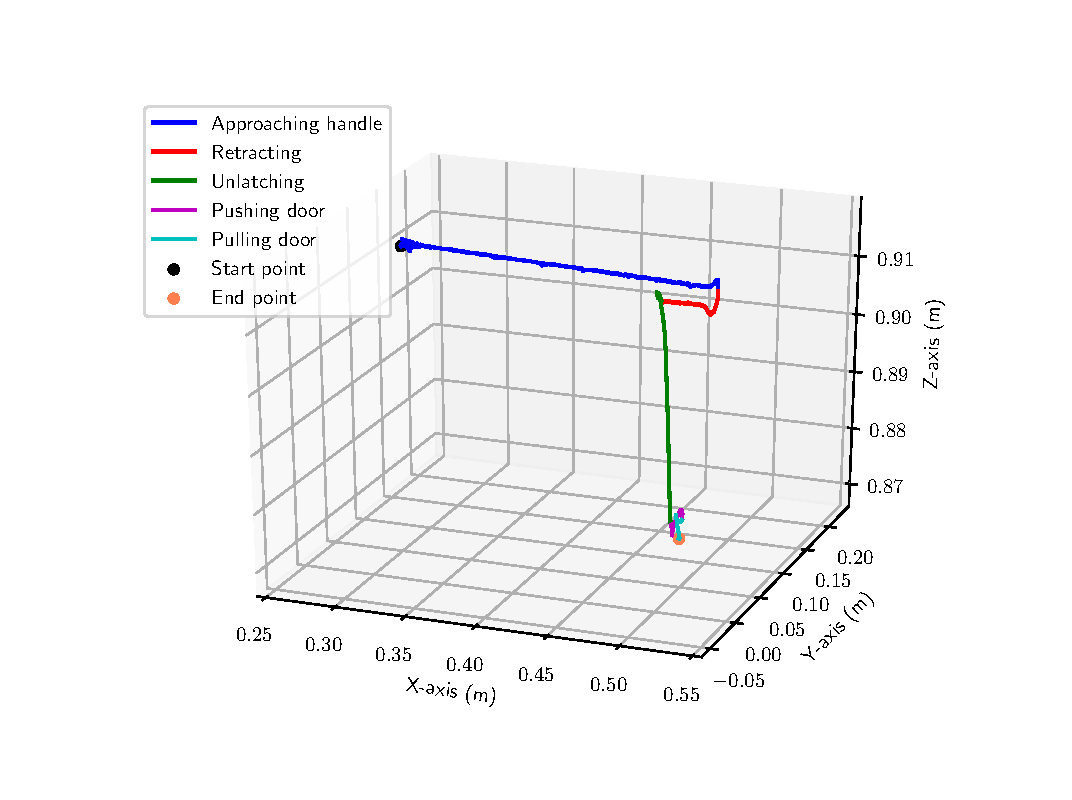
\includegraphics[width=0.8\textwidth]{images/exp/8776_traj.pdf}
		\caption{Geometric analysis of trajectory traced by TCP}

	\end{figure}
\end{frame}


\begin{frame}{~}{Discussion}
	\begin{itemize}
		
		\item Schunk LWA4D was able to open the door every time in 27 trials conducted.
				\item Robot was able to open the door in the presence of a bump on the floor.
		\item Toyota HSR robot was successful in detecting the opening direction of door and in determining whether the door is jammed or not.
		
		\item The chord length traced while opening door varies because :
		\begin{itemize}
			\item One or more joint limits reached
			\item Operation was stopped to avoid self-collision
		\end{itemize}
		\item Oscillations were observed in the trajectory because of :
		\begin{itemize}
			\item Drift in the sensor readings over time
			\item Delay in motion command update
		\end{itemize}

	\end{itemize}
\end{frame}


\begin{frame}{Vegetable Cutting Experiment}{\small Testing algorithm in simulation}
	\vspace{-0.5cm}
	\begin{itemize}
		\item Vegetable cutting task was simulated as motion of object through a viscous medium.
		\item REINFORCE algorithm successfully learned cutting policy.
	\end{itemize}
	\vspace{-0.6cm}
	\begin{figure}
		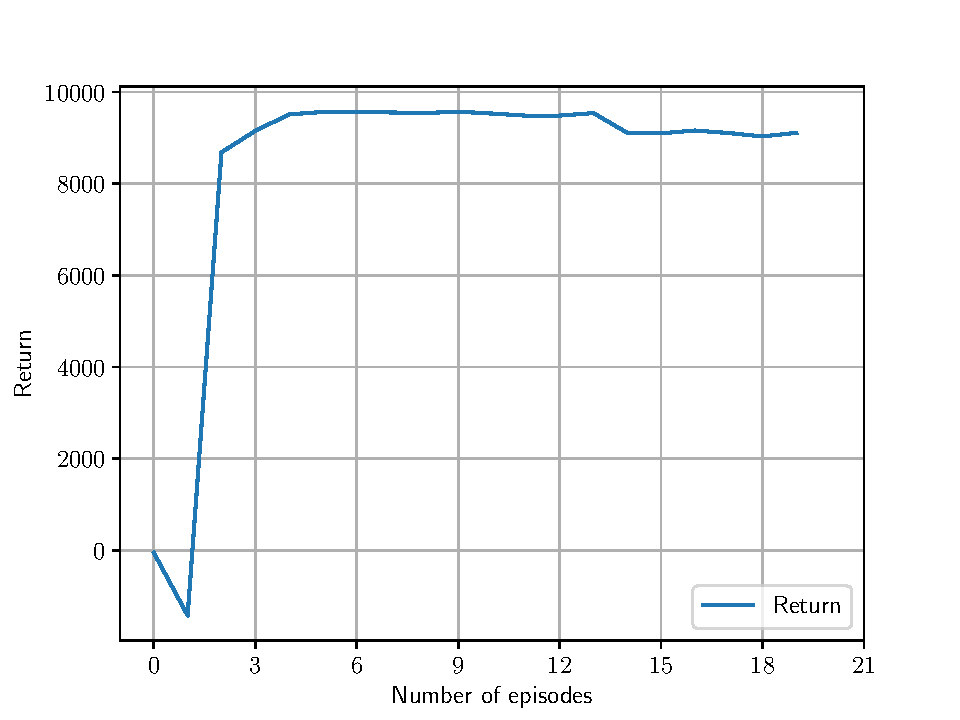
\includegraphics[width=0.6\textwidth]{images/exp/cut/sim_return}
		\caption{Performance of REINFORCE algorithm in simulation}
	\end{figure}
\end{frame}

\begin{frame}{~}{\small Experiments with KUKA LWR 4+}
	\begin{figure}
	\centering
	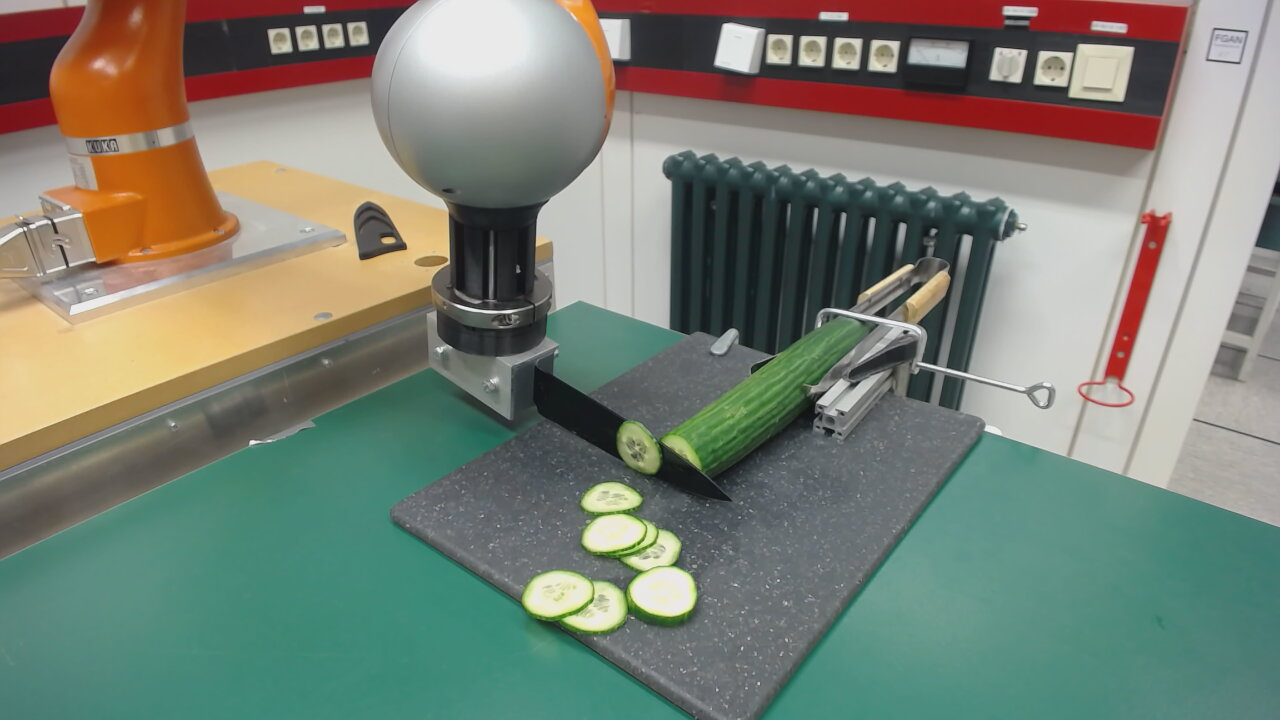
\includegraphics[width=0.85\textwidth]{images/exp/cut_veg_exp}
	\caption{KUKA LWR 4+ cutting vegetable}
	\end{figure}

\end{frame}

\begin{frame}{~}{\small Learning Force Policy with REINFOCE Algorithm}

	\newgeometry{textwidth=11.53cm}%
	%\vskip1ex
	\begin{minipage}[t]{0.51\textwidth}
		\begin{figure}
			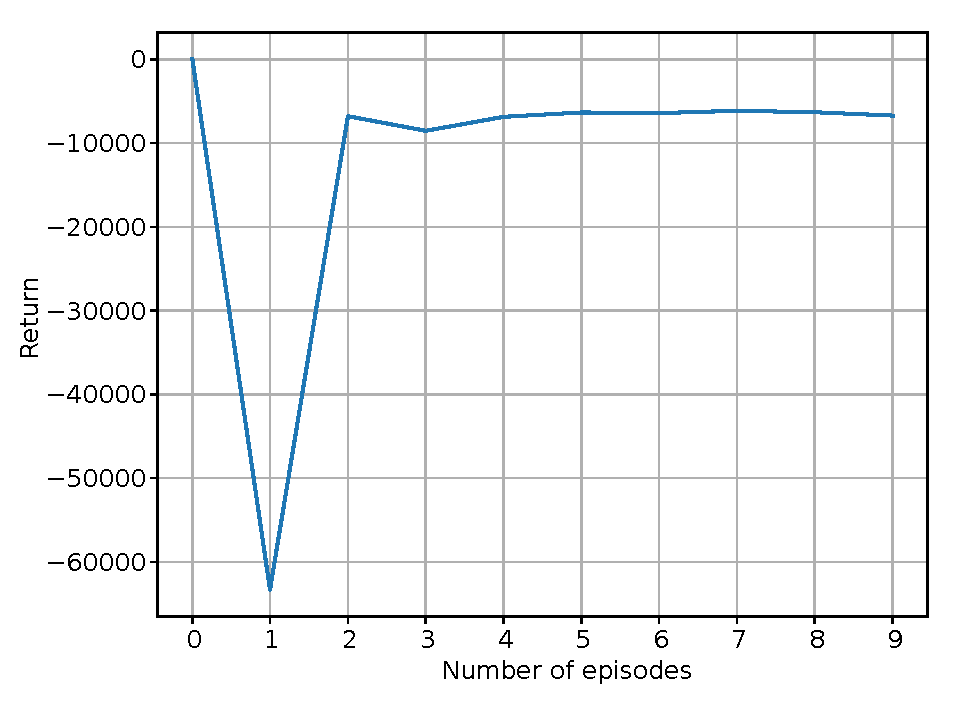
\includegraphics[width=0.95\textwidth]{images/exp/cut/reinf_returnn}
			\caption{\scriptsize Performance of REINFORCE algorithm with KUKA LWR 4+}
		\end{figure}
	\end{minipage}
	\hfill
	\begin{minipage}[t]{0.47\textwidth}
		\scriptsize
		\vspace{0.5cm}
		REINFORCE algorithm fails to learn force policy:
		\begin{itemize}
			\scriptsize 
			\item RINFORCE uses high frequency noise for exploration in action space
			\item The task and robot dynamics acts as a low-pass filter
			\item Contact dynamics also acts as low pass filter
			\item Hence noise is damped and REINFORCE does not converge.
		\end{itemize}
	\end{minipage}
\end{frame}

	
\begin{frame}{~}{\small Learning Force Policy with PoWER Algorithm}
	
	\newgeometry{textwidth=11.53cm}%
	%\vskip1ex
	\begin{minipage}[t]{0.51\textwidth}
		\begin{figure}
			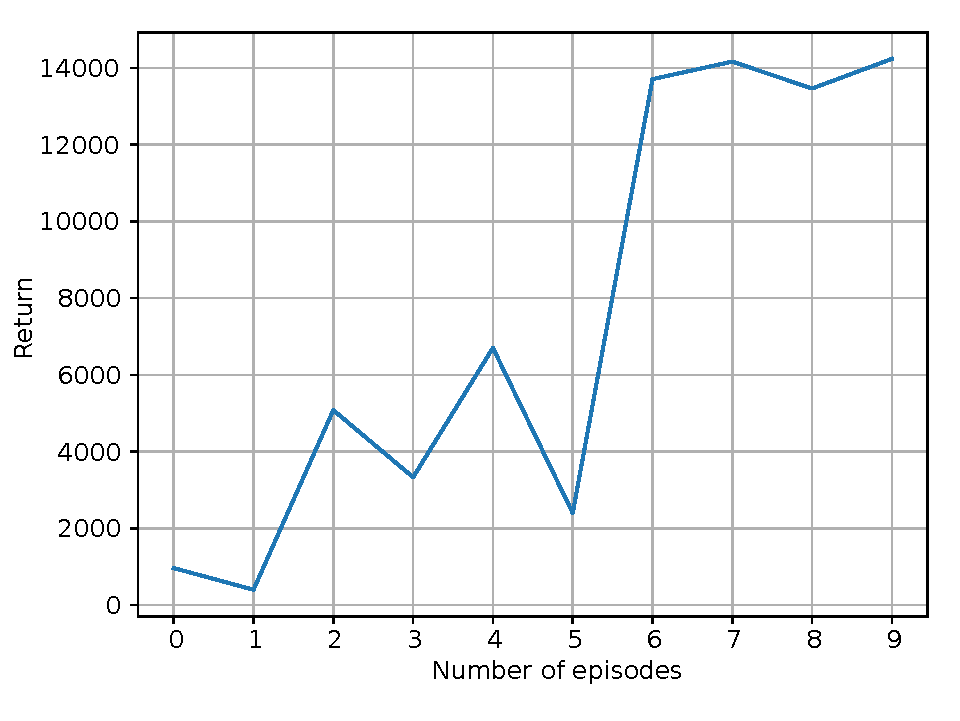
\includegraphics[width=0.95\textwidth]{images/exp/cut/power_return1n}
			\caption{\scriptsize Performance of PoWER algorithm with KUKA LWR 4+ using linear policy}
		\end{figure}
	\end{minipage}
	\hfill
	\begin{minipage}[t]{0.47\textwidth}
		\scriptsize
		\vspace{0.5cm}
		PoWER algorithm successfully learns force policy:
		\begin{itemize}
			\scriptsize 
			\item Policy was learned after 6 episodes
			\item Power uses low-frequency exploration noise
		\end{itemize}
	\end{minipage}
\end{frame}

	
	\begin{frame}{~}{\small Learning Force Policy with PoWER Algorithm}
		
		\newgeometry{textwidth=11.53cm}%
		%\vskip1ex
		\begin{minipage}[t]{0.49\textwidth}
			\begin{figure}
				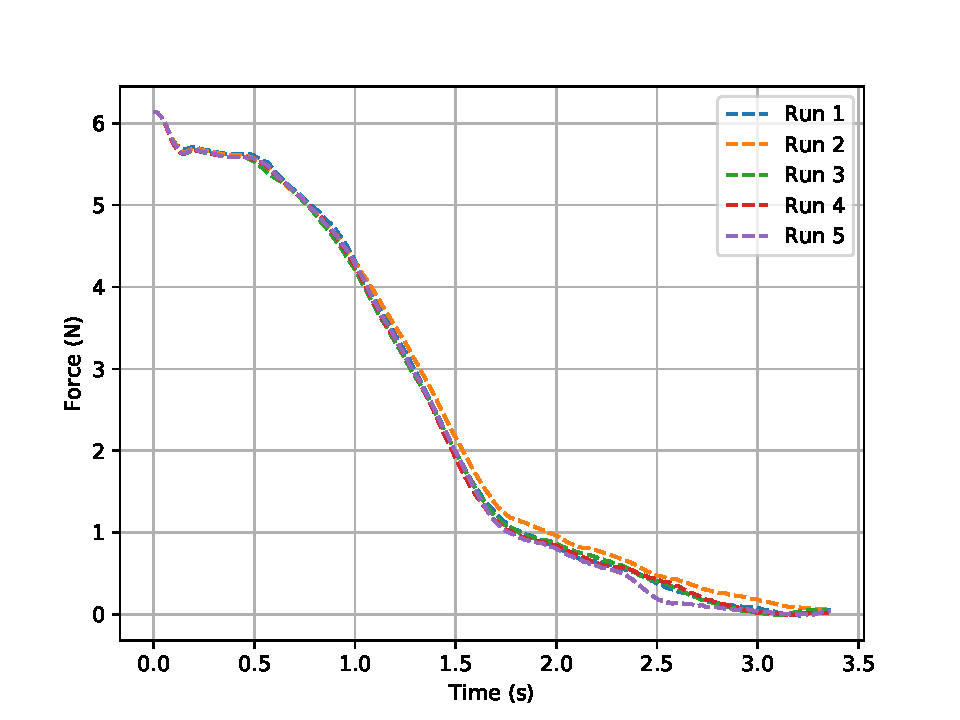
\includegraphics[width=\textwidth]{images/exp/cut/power_f1}
				\caption{\scriptsize Force generated by linear policy while cutting vegetable}
			\end{figure}
		\end{minipage}
		\hfill
		\begin{minipage}[t]{0.49\textwidth}
			
			\begin{figure}
				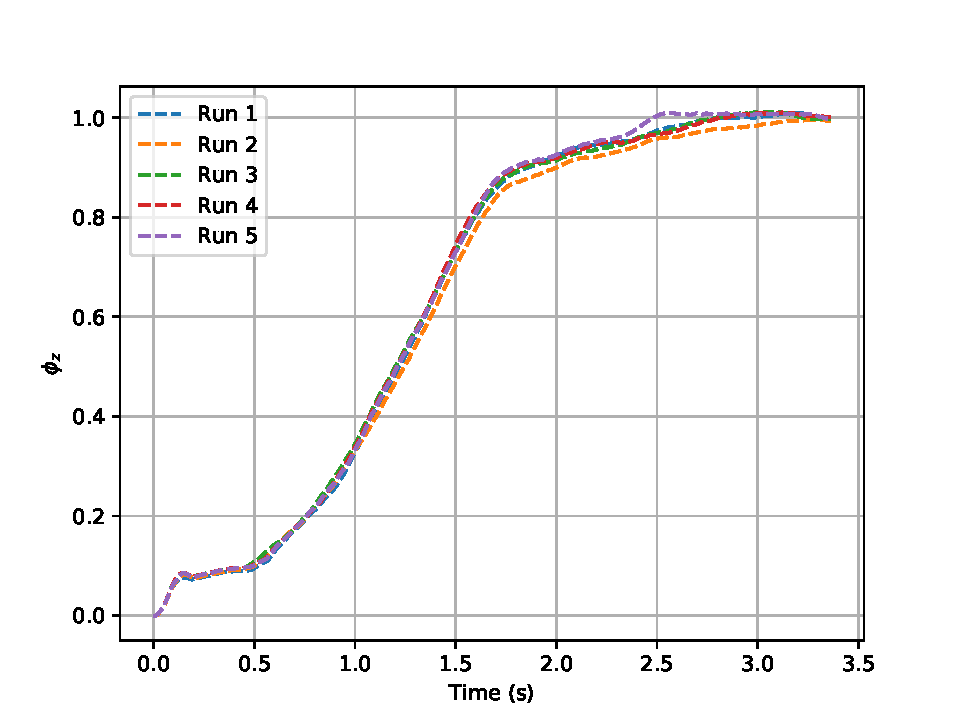
\includegraphics[width=\textwidth]{images/exp/cut/power_ph_z1}
				\caption{\scriptsize Cutting phase $\phi_{z}$ in Z-direction}
			\end{figure}
		\end{minipage}
	\end{frame}
	



\begin{frame}{~}{\small Learning Force Policy with PoWER Algorithm}
	
	\newgeometry{textwidth=11.53cm}%
	%\vskip1ex
	\begin{minipage}[t]{0.51\textwidth}
		\begin{figure}
			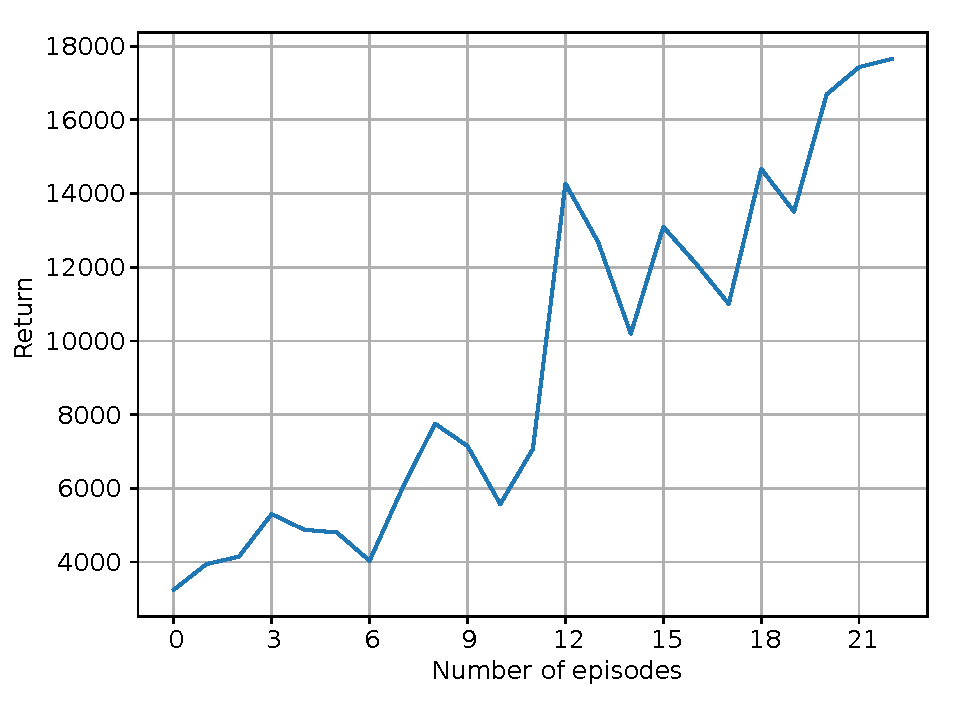
\includegraphics[width=0.95\textwidth]{images/exp/cut/power_return2n}
			\caption{\scriptsize Performance of PoWER algorithm with KUKA LWR 4+ using linear policy}
		\end{figure}
	\end{minipage}
	\hfill
	\begin{minipage}[t]{0.47\textwidth}
		\scriptsize
		\vspace{0.5cm}
		PoWER algorithm successfully learns force policy:
		\begin{itemize}
			\scriptsize 
			\item Policy was learned after 20 episodes
			\item Increase in number parameters requires more trials to learn the policy.
		\end{itemize}
	\end{minipage}
\end{frame}


\begin{frame}{~}{\small Learning Force Policy with PoWER Algorithm}
	
	\newgeometry{textwidth=11.53cm}%
	%\vskip1ex
	\begin{minipage}[t]{0.49\textwidth}
		\begin{figure}
			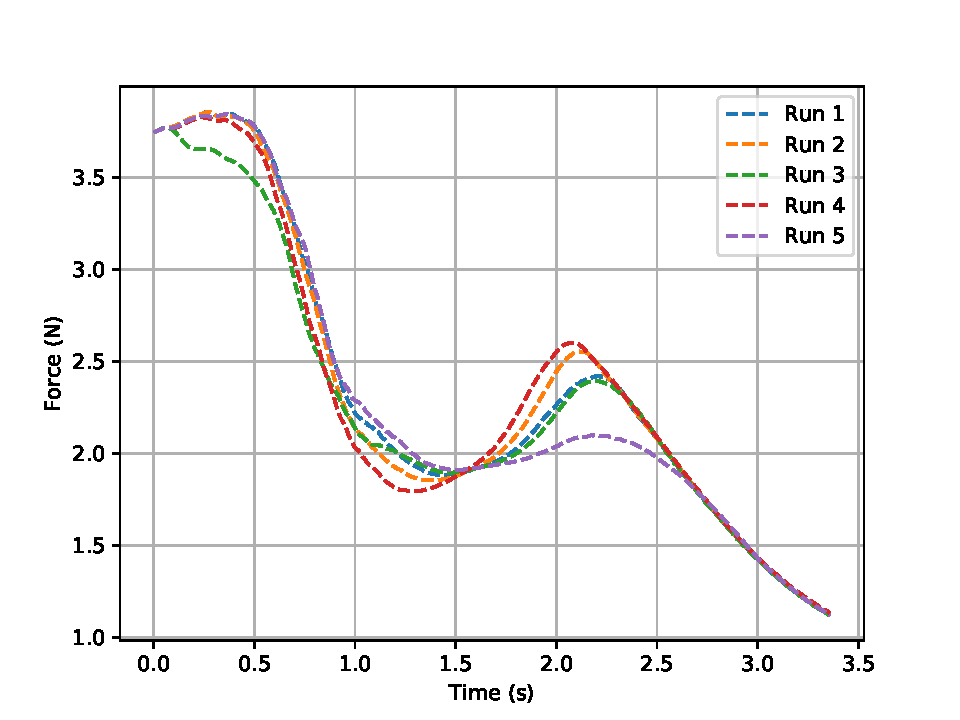
\includegraphics[width=\textwidth]{images/exp/cut/power_f2}
			\caption{\scriptsize Force generated by Gaussian policy while cutting vegetable}
		\end{figure}
	\end{minipage}
	\hfill
	\begin{minipage}[t]{0.49\textwidth}
		
		\begin{figure}
			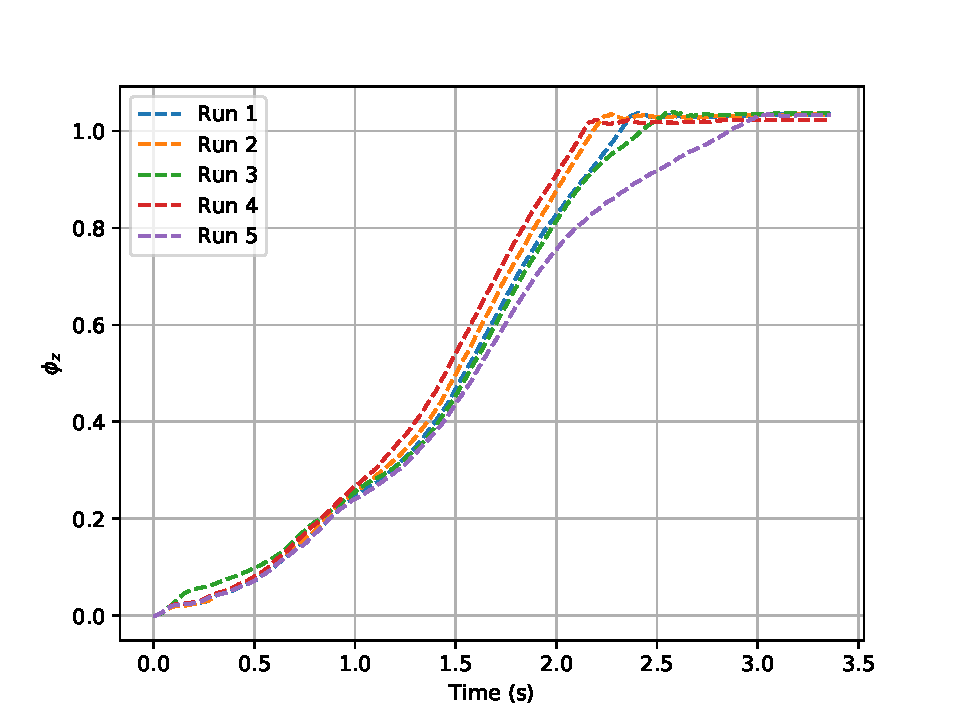
\includegraphics[width=\textwidth]{images/exp/cut/power_ph_z2}
			\caption{\scriptsize Cutting phase $\phi_{z}$ in Z-direction}
		\end{figure}
	\end{minipage}
\end{frame}




\begin{frame}{Conclusions}

%\vskip1ex

\begin{minipage}[t]{0.51\textwidth}
\begin{itemize}
\small 
\item A framework was developed for compliant manipulation using reinforcement learning guided by task specification. 
\item Task specification approach was successfully tested to solve door opening task using two different robots.
\item Evaluation of the task specification approach on two different robots proves the generalization capability of the approach.
\item We also extended the door opening solution to detect the opening direction of the door and if the door is jammed. 
\end{itemize}
\end{minipage}
\hfill
\begin{minipage}[t]{0.47\textwidth}
\begin{itemize}
\small
  
\item Oscillations were observed in the end-effector trajectory while opening door due to sensor noise and low command update rate.
\item Parameters of admittance controller were tuned to reduce the oscillations.

\end{itemize}
\end{minipage}
\end{frame}

\begin{frame}{Conclusions}
	
	%\vskip1ex
	
	\begin{minipage}[t]{0.51\textwidth}
		\begin{itemize}
			\small  
			\item Force policies for cutting vegetable were learned using PoWER algorithm with linear and Gaussian policy representation.
			\item Policies were learned directly on the robot, without using simulation.
			\item It was also observed that the cutting depth achieved in previous trial affected the return of the next trial due to more resistant provided by vegetable.
			\item Task specification framework reduced the dimensions of the problem from six to one, which resulted in faster learning directly on the robot.
		\end{itemize}
	\end{minipage}
	\hfill
	\begin{minipage}[t]{0.47\textwidth}
		\begin{itemize}
			\small 
			\item REINFORCE algorithm failed to learn force policy for cutting vegetables because of ineffective exploration with high frequency noise in low-pass filter like environment.
			\item Increase in policy parameters resulted in increase in number of trials required for learning.
			\item simple policies can be very effective when one is interested in learning to perform the task rather than learning the complex dynamics of the environment in which the task is being performed.
		\end{itemize}
	\end{minipage}
\end{frame}

\begin{frame}{Future Work}
	
	%\vskip1ex
	
	\begin{minipage}[t]{0.51\textwidth}
		\begin{itemize}
			\small  
			\item Auto-tuning for tuning of admittance controller parameters.
			\item Extending the approach for tasks such as sweeping the floor, cutting curtains and bags during an investigation of the potentially dangerous environment.
			\item Extending  for tasks involving multi-directional force interactions with the environment such as collaborating with human to transport objects from one place to another.
		\end{itemize}
	\end{minipage}
	\hfill
	\begin{minipage}[t]{0.47\textwidth}
		\begin{itemize}
			\small 
			\item Reducing the delay in ROS communication.
		\end{itemize}
	\end{minipage}
\end{frame}

\begin{frame}[allowframebreaks]{References}
	
	\bibliography{../../project-proposal/bibliography}
	\bibliographystyle{abbrv}
	
\end{frame}

\end{document}
